\documentclass{scrartcl}

\usepackage{amssymb}
\usepackage{amsmath}
\usepackage{tikz}
\usetikzlibrary{calc}					%for centerarc
\usetikzlibrary{decorations.text}		%for bendy superego
\usetikzlibrary{arrows, arrows.meta}	%for big arrowheads in topography #1

\def\centerarc[#1](#2)(#3:#4:#5)% Syntax: [draw options] (center) (initial angle:final angle:radius)
{ \draw[#1] ($(#2)+({#5*cos(#3)},{#5*sin(#3)})$) arc (#3:#4:#5); }

\begin{document}
	
	\hspace{0.5cm}
	%\begin{figure}
	%	\centering
	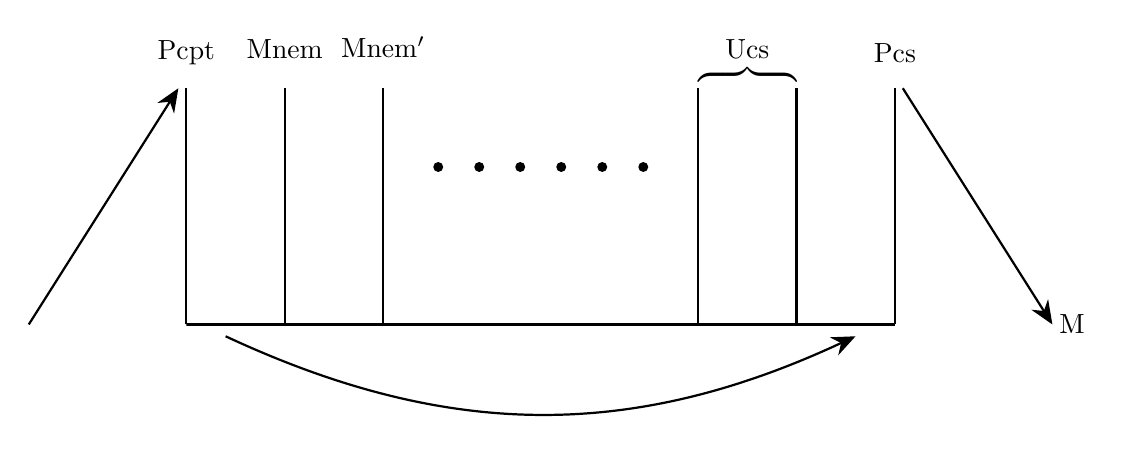
\begin{tikzpicture}
	\draw[thick] (0,0) rectangle (9,0);		%horizontal line
	\foreach \x in {0,...,5} 
	\fill (3.2+\x/1.92,2) circle (1.8pt);	%dots
		
	%vertical lines, left
	\draw[thick] (0,0)--(0,3);
		\node at (0,3.45) {Pcpt};
	\draw[thick] (1.25,0)--(1.25,3);
		\node at (1.25,3.5) {Mnem};
	\draw[thick] (2.5,0)--(2.5,3);
		\node at (2.5,3.52) {Mnem$^\prime$};
	
	%vertical lines, right
	\draw[thick] (6.5,0)--(6.5,3);
	\draw[thick] (7.75,0)--(7.75,3);
		\node at (7.125,3.15) {\rotatebox{270}{$\left\{ \rule{0pt}{7mm}\right.$}};
		\node at (7.125,3.5) {Ucs};
	\draw[thick] (9,0)--(9,3);
		\node at (9,3.45) {Pcs};
	
	%arrows
	\draw[-{Stealth[length=3mm,width=2.5mm]}, thick]	(0.5,-0.15) to[bend right=25] (8.5,-0.15);
	\draw[-{Stealth[length=3mm,width=2.5mm]}, thick]	(-2,0)--(-0.1,3);
	\draw[-{Stealth[length=3mm,width=2.5mm]}, thick]	(9.1,3)--(11,0);
		\node at (11.25,0) {M};
	\end{tikzpicture}
	%	\caption{Freud's first topography}
	%\end{figure}
	
	
	\vspace{1.5cm}		%this is to make all 3 diagrams fit on one page
	
	
	%\begin{figure}
	%	\centering
	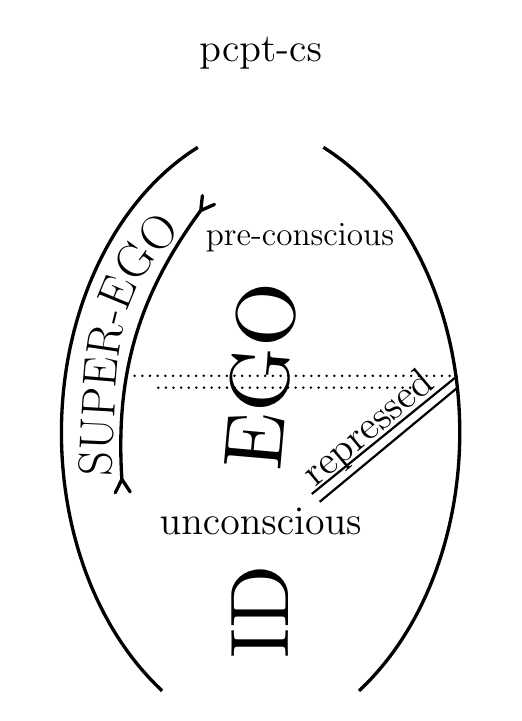
\begin{tikzpicture}
	%top part
	\centerarc[very thick](0,6.5)(-10:190:1.25)
		\node at (0,8.1) {{\Large pcpt-cs}};
	
	%side arcs
	\draw[very thick] (-1.25,0) arc (235:115:3cm and 4cm);	%left arc
	\draw[very thick]  (1.25,0) arc (-55:65:3cm and 4cm);	%right arc
	
	%inside small arc
	\draw [<->,>=angle 60 reversed, very thick]	(-1.75,2.5) to[bend left=20] (-0.65,6.25);
	\draw [decorate, decoration={text along path, text align=center, text={|\LARGE|SUPER-EGO}}] (-1.9,2.5) .. controls (-1.8,5) .. (-0.85,6);
	
	%labels
	\node at (0.5,5.75) {{\large pre-conscious}};
	\node[scale=3] at (0,1) {\rotatebox{90}{ID}};
	\node[scale=3] at (0,4) {\rotatebox{85}{EGO}};
	\node at (0,2.15) {{\Large unconscious}};
	\node at (1.38,3.32) {\rotatebox{40}{{\Large repressed}}};
		\draw[thick]  (0.65,2.5)--(2.5,4);
		\draw[thick]  (0.75,2.4)--(2.5,3.85);
	%
	\foreach \x in {0,...,41} 						%upper dotted line
	\fill (-1.6+\x/10.25,4) circle (0.5pt);			%(2.5,4)--(-1.6,4)
	%
	\foreach \x in {0,...,33} 						%(1.9,3.85)--(-1.3,3.85)
	\fill (-1.3+\x/10.3125,3.85) circle (0.5pt);	%33/(1.3+1.9) = 10.3125
	%
	%NB: in the original German diagram, the dotted line goes from one side to the other
	\end{tikzpicture}
	%	\caption{Freud's second topography}
	%\end{figure}
	%
	%
	\hspace{1.5cm}
	%
	%
	%\begin{figure}
	%	\centering
	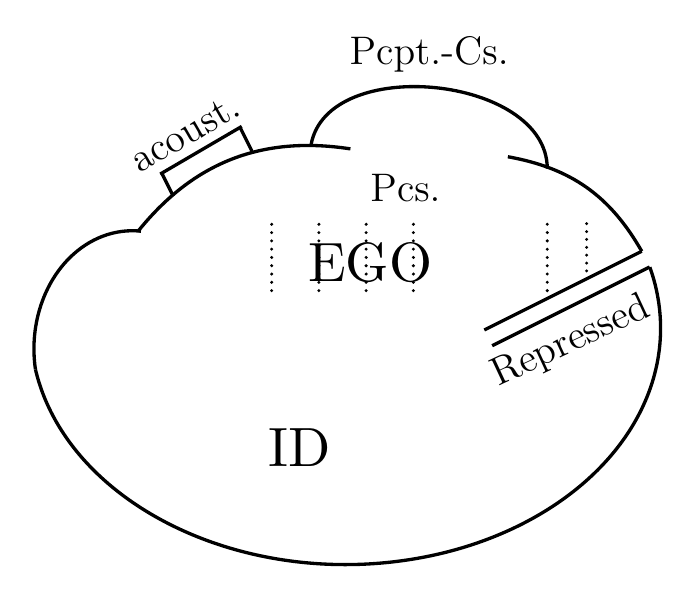
\begin{tikzpicture}
	\draw[very thick] (0,0) arc (190:375:4cm and 3cm);		%bottom arc
	\draw[very thick] (0,0) arc (190:85:1.25cm and 1.5cm);	%sticky-outy part
	\draw[very thick] (1.3,1.75) to[bend left=30] (4,2.8);	%top-left arc
	\draw[very thick] (7.7,1.5) to[bend right=25] (6,2.7);	%top-right arc
	\draw[very thick] (3.5,2.85) to[out=80,in=90] (6.5,2.55);
	
	%lines
	\draw[very thick] (7.8,1.3)--(5.8,0.3);		%lower line
	\draw[very thick] (7.7,1.5)--(5.7,0.5);		%upper line
	%box
	\draw[very thick] (1.75,2.20)--(1.6,2.5);	%left line
	\draw[very thick] (2.75,2.77)--(2.6,3.07);	%right line
	\draw[very thick] (1.585,2.48)--(2.62,3.085);	%top line
	
	%labels
	\node[scale=2] at (3.35,-1) {ID};
	\node[scale=2] at (4.25,1.35) {EGO};
	\node at (4.7,2.3) {{\Large Pcs.}};
	\node at (5,4) {{\Large Pcpt.-Cs.}};
	\node at (1.9,3) {\rotatebox{30}{{\Large acoust.}}};
	\node at (6.8,0.35) {\rotatebox{25}{{\Large Repressed}}};
	
	%dotted lines
	\foreach \x in {0,...,6} 
	\fill (7,1.25+\x/10) circle (0.6pt);		%rightmost line (7,1.25)--(7,1.85)
	\foreach \x in {0,...,8} 
	\fill (6.5,1+\x/9.5) circle (0.6pt);		%second from right (6.5,1)--(6.5,1.85)
	%
	\foreach \x in {0,...,8} 
	\fill (4.8,1+\x/9.5) circle (0.6pt);		%rightmost in middle: (4.8,1)--(4.8,1.85)
	\foreach \x in {0,...,8} 
	\fill (4.2,1+\x/9.5) circle (0.6pt);		%(4.2,1)--(4.2,1.85)
	\foreach \x in {0,...,8} 
	\fill (3.6,1+\x/9.5) circle (0.6pt);		%(3.6,1)--(3.6,1.85)
	\foreach \x in {0,...,8} 
	\fill (3,1+\x/9.5) circle (0.6pt);			%leftmost line (3,1)--(3,1.85)
	\end{tikzpicture}
	%	\caption{Freud's second topography}
	%\end{figure}
	
\end{document}
